%! program = pdflatex

\documentclass[11pt]{article}
\usepackage[margin=1in]{geometry}
\usepackage[medium,compact]{titlesec}
%\geometry{a4paper} % or letter or a5paper or ... etc
% \geometry{landscape} % rotated page geometry

\usepackage{graphicx}
\usepackage{caption}
\usepackage{subcaption}
% See the ``Article customise'' template for come common customisations

\title{Shelf Unique IP: Provisional Patent Claims + Trade Secret}
\author{Lauren Jung\\Shelf Inc. \and Atul Singh\\Shelf Inc.}
\date{} % delete this line to display the current date





%%% BEGIN DOCUMENT
\begin{document}

\maketitle
%\tableofcontents

\abstract{Systems and methods are disclosed for analysis and inference of promotions sent by retailers; to find the lowest price and availability of retailers items; to recommend ways to redeem promotions.}
%; to recommend new promotions based on a user's selection of items; and recommending time to buy an item.}

\section{Claim: A system to discover, analyze, and infer promotions}

\textbf{Input:}\\
Retailer Promotion Sources (Web URL, promotional email, social media URLs)\\

\noindent
\textbf{Output:}\\ A list of promotions, each a tuple containing:\\
$<$Discount info (type, code, discount value, threshold)$>$, $<$Validity$>$, $<$Availability$>$, $<$Applicability$>$\\

\noindent
Type = \{Store-wide, Buy1-Get1, Aggregate, Shipping\}\\
Code = \{alpha-numeric or None\}\\
Discount value = \{E.g., 20\%\}\\
Threshold = \{E.g., \$100 for a promotion ``Spend \$100 to Save \$25"\}\\
Validity= \{Start-date, End-date\}\\
Availability = \{In-store, Online, Both\}\\
Applicability = \{Everything, Category list, Excludes\}\\


\paragraph{High-level idea}
We first get the raw information from the sources (email, HTML from the store's online pages as well as Facebook/Twitter feeds) and find out promotion related information in 
easy to analyze textual format. This requires us to parse the information present in different syntaxes (HTML, email, images)
to a common format. Next, the raw input is parsed and mapped to a set of promotion rules using machine-learning based pattern matching
algorithm. Figure~\ref{fig:claim1} captures this.

\begin{figure}[htbp]
\begin{center}
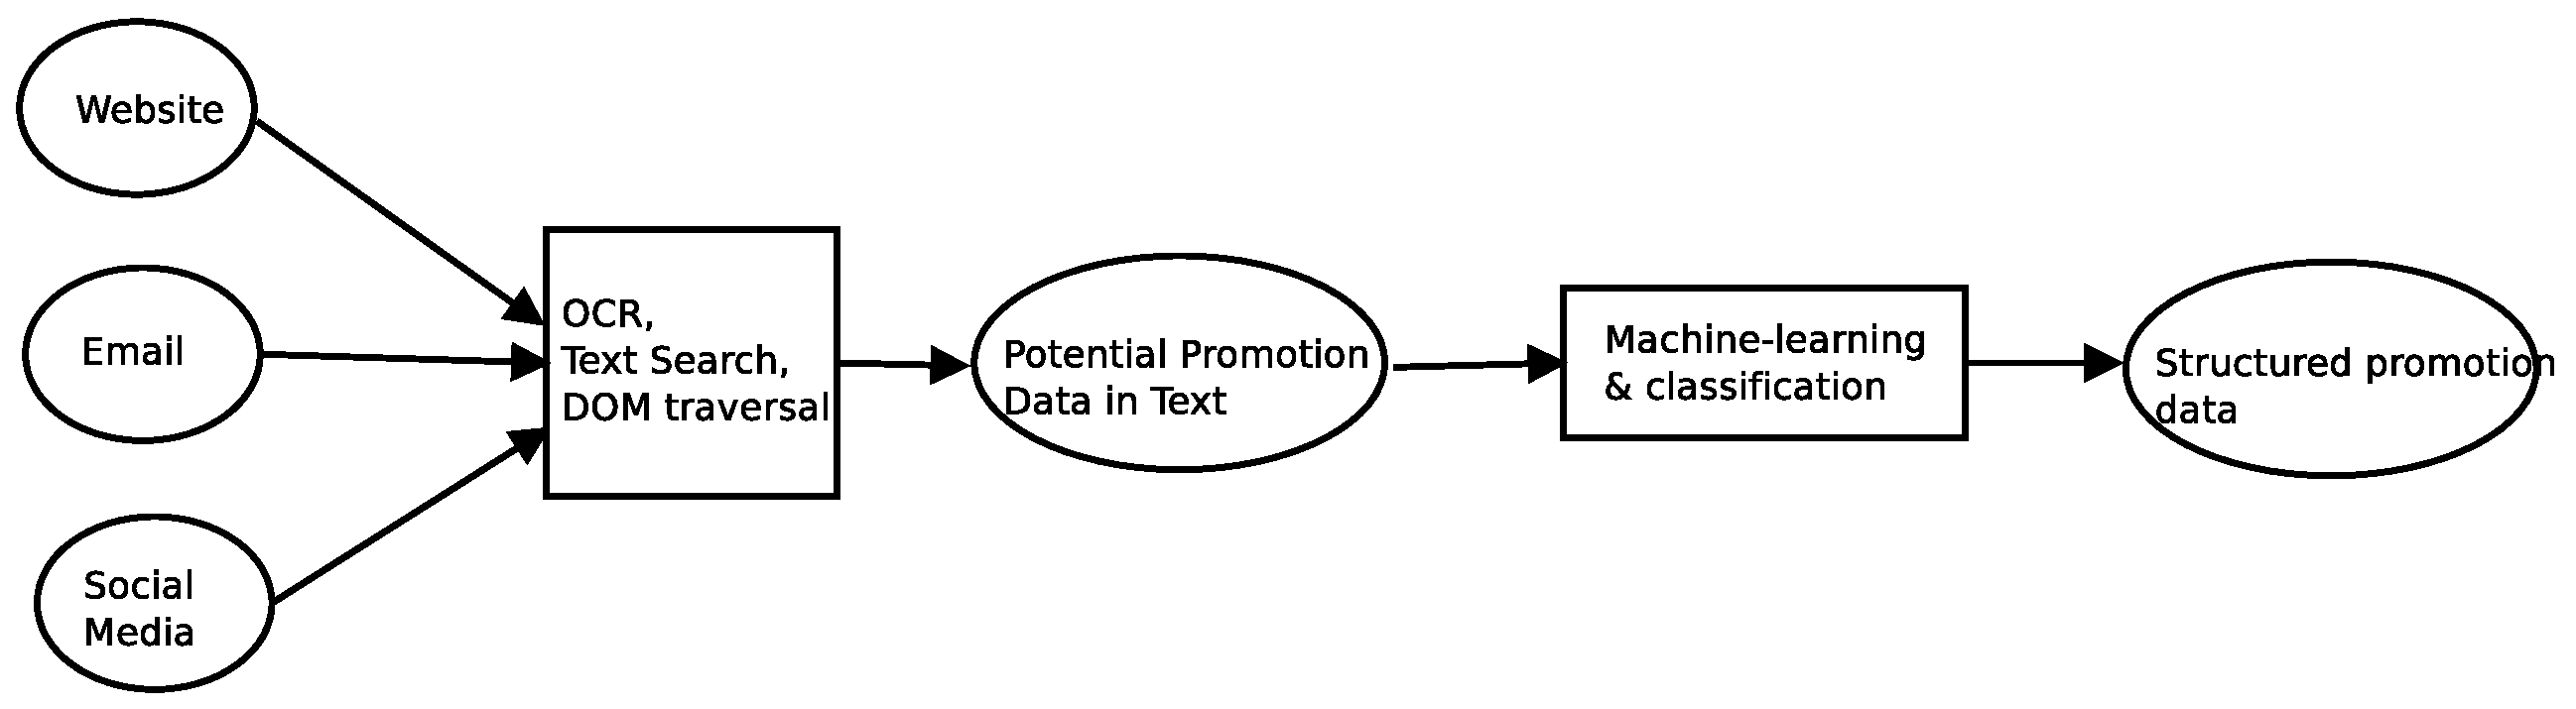
\includegraphics[width=\textwidth]{claim1}
\caption{High-level idea.}
\label{fig:claim1}
\end{center}
\end{figure}



\subsection{Raw-input to text translation}

\paragraph{For Web URL source (similar for other sources)} Start:\\
a) Crawl the home page using a standard off-the-shelf web browser emulator (such as Selenium) to crawl the Web URL\\
b) Find all leaves of the DOM tree of the web-page that contain some text inside\\
c) Filter out leaves that contain promotion-related keywords \{promotion, discount, off, save, sale, shipping, sale, season, \$, \%\}\\
d) For each such leaf: find the sibling DOM elements and their associated text or image (this forms a promotion unit)\\
e) Find all image elements in the DOM, and for each image, obtain the value of the "alt", "title" text values, id of the "area" map, and click on sibling or children nodes that have text "see details", "details", "more"\\
f) Find the DOM element of type area with the id found in the previous step, get it's "href" tag and store it in the next URL to visit next\\
g) For each image found, perform OCR using a standard off-the-shelf OCR solution (e.g., Google's Tessaract) to extract text from the image (this forms a promotion unit as well)\\
h) Repeat the above steps for the content obtained by visiting the URL's in the next list



Output of this step is a set of promotion units: a set of text-lines containing potential promotion information.

\subsection{Text-to-promotion-rule classification}



At a high-level, our algorithm uses decision-tree based machine-learning algorithms to perform automatic classification of text-based promotion units to structured promotion data (or a promotion rule). A promotion rule, as described above, consists of:\\
$<$Discount info$>$, $<$Validity$>$, $<$Availability$>$, $<$Applicability$>$

\paragraph{Attributes:} We have identified following attributes:\\
Discount related: \{buy 1, buy one, get, off, a number, spend, free, sale, clearance, shipping, use code, code, use, \$, \%,\}\\
Validity related: \{valid, last, day, tick, tock, (any) day of the week, (any) month of the year, limited time, today, \}\\
Applicability related: \{everything,  $<$category name$>$, men, women, boys, kids, girls,\}\\
Availability related: \{store, online, both\}\\

Next, we searched for these attributes in the potential promotion units found in the previous section. The output of this process is a list of vectors, each corresponding to a potential promotion unit. A vector for a token corresponds to the values assigned to the different attributes found in its text. The results are presented in a special format .arff, so that they can be directly processed by most machine learning tools, such as Weka. 

%The text we have obtained so far is in some sense high level summary. What about the fine print? Sometimes fine-print doesn't contain all the information.

%Challenges:
%a) heterogeneity
%b) completeness
%c) accuracy
%d) promptness

%Pattern recognition algorithm then finds out the relation between different attributes to know what values of these attributes 

%Idea1: do it for couple of stores and then generalize it to arbitrary stores
%Idea 2: look at the fine-print
%\begin{enumerate}
%\item Text => Promo Rule Template mapping (machine learning to do pattern recognition) 
%\item Rule template => Rule generation (fill the details)
%\end{enumerate}

%Question: why not simple grep or regular expression? We tried that first and it worked OK in the beginning. But the syntax changes and different stores have slightly different syntax. 

%Once we know what promotion type it is, we can then search for values to fill the rule template.

\section{Trade Secret: Automatic Promotion Application and Availability Testing}

\paragraph{Input:} 
- Product URL\\ 
- html tags for color/size elements for the store\\ 
- html tags for add-item-to-cart for the store\\
- html tags for checkout for the store\\
- html tags for element that is needed for adding promo code for the store\\

\paragraph{Output:} for the given product:\\
a) current lowest price for each color/size,\\
b) applicable promotion code (if any),\\
c) availability for each color/size
 

\paragraph{Algorithm:} Our algorithm consists of following steps:\\
- Start an Internet browser (like Firefox) by invoking Selenium, a browser automation system\\
- Visit product url\\
- Find all colors (finding the list of selectable items on the page for the color specific elements)\\
- For each color, click on it (or select it) and observe the available sizes and prices (after refreshed by the browser)\\
       			-This gives us the {availability, base price} for color/size\\
   		- Select a random color and a random size combination\\ 
       		- Add item to the cart by clicking on 'add-to-cart' button\\
   		- Save the current price\\
       		- Enter each promotion code (obtained from the algorithm of claim \#1) to the html DOM element for entering promotion code\\
   	     	- Get the final price and calculate savings due to the promo code\\
		- Remove the promotion code and repeat if there are more promotion codes left


\section{Claim 2: Recommendation of Ways to Redeem Promotions}

\subsection{Aggregate Type of Promotions}
\paragraph{Input:} A promotion $P$ of type Aggregate (e.g.: ``Spend X and Save Y: X $>$ Y") from retailer A and a set of items from retailer A.

\paragraph{Output:} for each item, maximal savings achieved due to the promotion.\\


\paragraph{Algorithm:} Our algorithm consists of following steps:\\
\begin{tabbing}
For each item i in items:\\
if item\=.price $>$ X:\\
\> savings.amount = Y\\
\> savings.promo = $P$\\
\> savings.required\_item = None\\
\> item.savings = savings\\
\> continue\\
if item.price $>$ X-Y:\\
\> diff = X - item.price\\
\> // save 25 off \$100. Item is 80, so diff = 20, Y =25. So, we end up saving \$5\\
\> // this is a feasible space where a user can spend diff and save Y, so overall a savings of Y-diff\\
\>find an item $\delta$ from retailer A such that $\delta$.price $\ge$ diff $\wedge$ $\delta$.price is minimum\\
\> // suggest user to buy this item and become eligible for redeeming this promotion\\
\> savings.amount = (Y - $\delta$.price)\\
\> savings.required\_item = $\delta$\\
\> savings.promo = $P$\\
\> item.savings = savings\\

\end{tabbing}

\subsection{B1G1 Type of Promotions}

\paragraph{Input:}  A promotion $P$ of type B1G1 (e.g.: ``Buy 1 Jeans, and get another at 50\% off") from retailer A, a user $U$ of Shelf, list of items the user is interested in (for buying) from retailer A, and $U$'s online social network $S$ (friends, family: connected via email or online social network) present on Shelf.


\paragraph{Output:} List of item-sets.\\


Basic idea is to find other items that are required for activating the promotion. We first search in the list of items $U$ has shelved and then search
in the list of items $U$'s social network has shelved.

\paragraph{Algorithm:} Our algorithm consists of following steps:\\
\begin{tabbing}	
$C$ = $P$.category\\
threshold = $P$.threshold\\
//testing if promotion $P$ works on an item is our trade secret: can we re-use this?\\
items\_\=eligible = items from retailer A shelved by $U$ and promotion $P$ works on them\\
if num(items\_eligible) $\ge$ threshold:\\
\>result = find subsets of size threshold from items\_cat\\
\>return ($U$, result)\\
else:\\
\>// Not enough items shelved by $U$, so should look at friends items next\\
\>result\_set = ()\\
\>for \=user $F$ in $S$:\\
\>\> item\_eligible\_$F$ =\=  items shelved by $F$ and promotion $P$ works on them\\
\>\> if num\=(items\_eligible\_$F$) $\ge$ threshold:\\
\>\>\>result = find subsets of size threshold from items\_eligible\_$F$\\
\>\>\>add ($F$, result) to result\_set\\
\>sort result\_set based on variety of settings: price-based, popularity-based, or by interest-based\\ 
\>return result\_set\\


\end{tabbing}

\if 0
\section{Claim 3: Recommendation of New Promotions}
Prior art: recommendation for new products is everywhere based on this history of products you buy
- what worked in the past
- what our competitors are doing


Our insight: combination of
a) historical items a user has bought in the past
b) based on the items they have in their Shelf (from them or their competitors)
c) based on the kind of promotions they have utilized in the past
d) based on their friends
e) price points users have set in their alerts


\section{Claim 4: Recommend a time to buy an item} 
Prior art: based on historical price fluctuations (in stock market)
decide.com: + blogs, company news, etc.

What is our insight that will make us provide better recommendation?
--they don't do it for apparel yet (only electronics)
--in apparel: mid-season price fluctuations happen because of promotions
--promotions are sent because of a variety of reasons: what competition is doing

\fi
\end{document}